In virtù delle mancanze del tool SMART delineate nel Capitolo 5, si è deciso di procedere alla realizzazione di un'applicativo web ad hoc per sopperire alle lacune del suddetto tool.

\vspace{3mm}

Il tool in sviluppo, denominato LW Index, in riferimento all'omonima metrica presentata nel Capitolo 2, è definito come SMART-like, o simil-SMART. Il tool SMART permetteva di confrontare una serie di algoritmi di confronto fra stringhe, a prescindere dalla loro natura, e generare conseguentemente dei grafici predisposti a valutazioni di natura qualitativa da parte dell'utente.

Benché sia disponibile in una versione parallela adoperante un'interfaccia grafica, SMART nasce come programma da terminale; nella fattispecie, come si è osservati nel Capitolo 4, è in grado di produrre - a partire da una collezione di stringhe (o più banalmente un testo) e uno spettro di algoritmi selezionati - una pagina web costruita tramite elementi di HTML, CSS e JavaScript. 

D'altro canto, l'interazione dell'utente nasce e muore nel contesto del terminale: difatto, la pagina web autogenerata da SMART è di mera consultazione e non prevede ulteriore interazione con l'utente.

\vspace{3mm}

L'obiettivo è dunque di creare un tool che riesca ad accogliere algoritmi basati sulla metrica LW, incompatibili coi metodi di elaborazione e computazione di SMART; si noti, in ogni caso, che la metrica LW e le \textit{minimal absent words} sono strettamente legate, motivo per cui il tool è stato pensato specificamente per algoritmi che, oltre a misurare la similitudine con la metrica LW, facciano uso di \textit{minimal absent words} e derivati nella loro composizione funzionale.

\section{Progettazione del tool}

    Si osservi che, d'ora in poi, l'espressione "tool in sviluppo" sarà utilizzata in maniera intercambiabile col suo proprio nome, quale LW Index. 

    \subsection{Caratteristiche e funzionalità ad alto livello}

        In generale, il tool in sviluppo permetterà di creare grafici (al più 4) in maniera del tutto simile al tool SMART; svuotare la tavola di lavoro (cioè distruggere i grafici--tutti o individualmente) e analizzare i grafici. Creare un grafico significa, ad alto livello, generare un'istanza di lavoro vuota, popolabile con dati e stringhe durante la fase di analisi. 
        
        Analizzare i grafici significa porre in evidenza uno dei grafici fra quelli creati sulla tavola di lavoro ed effettuare una serie di azioni, fra cui visionare, in maniera grafica o testuale, il processo computazionale svolto per arrivare a quei dati, e modificare i grafici aggiungendo, rimuovendo o alterando stringhe. 
        
        \vspace{3mm}
        
        E' importante sottolineare che modificare il grafico significa necessariamente creare una nuova richiesta computativa.
        
        \vspace{3mm}
        
        Sarà possibile cambiare algoritmo. Il tool sarà sufficientemente versatile da accogliere un insieme diversificato di algoritmi che hanno in comune l'impiego della stessa metrica di similitudine fra stringhe, quale l'indice LW.
 
        \vspace{3mm}
 
        I grafici rappresenteranno sulle ascisse le stringhe (su alfabeti ben definiti) e sulle ordinate il corrispettivo indice LW. Questo significa che, per ogni stringa, il grafico produrrà una curva distinta a cui assocerà un indice LW per ogni altra stringa di quel grafico.  
        
        Come accennato, il tool potrà ospitare al più 4 grafici per volta, ed ogni grafico sarà analizzabile e modificabile indipendentemente dagli altri.

    \subsection{Architettura dell'applicazione}
    
        Il tool LW Index adotterà un'architettura web di tipo client-server. L'utente si interfaccerà con l'applicazione attraverso un browser web come Google Chrome o Mozilla Firefox. Questa scelta risulta funzionale perché il tool dovrà offrire un maggior numero di opzioni d'interazione rispetto a SMART, e preservare i dati fra un'esecuzione e l'altra.
        
        \vspace{3mm}
        
        Gli algoritmi di confronto dovranno essere ospitati sul server in una specifica directory. 
        
        \vspace{3mm}
        
        Nel dettaglio, l'utente potrà avviare l'applicativo tramite terminale. Una volta lanciato uno specifico comando, un'istanza del client (ossia una pagina web) si aprirà e contemporaneamente il webserver si avvierà.
        
        \vspace{3mm}
        
        Fra le caratteristiche proposte al punto 5.1.1, l'unica funzionalità che richiede l'intervento del server è la modifica di un grafico. Si noti che, pure se un grafico è vuoto (e cioè non è stato ancora popolato da stringhe), si sta affrontando un'operazione strettamente di modifica. Ogni volta che si richiede di aggiungere, eliminare o modificare stringhe, e si avvia il processo computativo alla pressione di un tasto, il webserver dovrà essere contattato e informato sulla natura della richiesta, per poi trattare i dati in put ed eventualmente fornire in output i dati necessari alla generazione del grafico.
    
    \subsection{Scelta delle tecnologie impiegate nell'implementazione}
    
        L'applicativo sarà implementato con tecnologie moderne e convenienti, al fine di semplificare la fase di implementazione e ridurre al minimo i casi di errore da gestire. Si è dunque deciso di implementare il webserver e il backend dell'applicazione con Node, mentre il frontend del client con React. Il techstack costituito da React e Node è un'alternativa popolare all'utilizzo grezzo della tecnologia fondamentale dalla quale entrambi derivano, quale JavaScript. 
        
        \vspace{3mm}
        
        Per ciò che concerne il frontend, le applicazioni web implementate in React possono sfruttare JavaScript o TypeScript; quest'ultimo, notoriamente, è un'alternativa al primo ed è caratterizzato da una forte tipizzazione, del tutto mancante invece in JavaScript. 
        
        E' stato deciso di implementare il tool in sviluppo con la variante TypeScript di React.
        
        \vspace{3mm}
        
        Per ciò che concerne il backend, Express, popolare framework di Node, è stato selezionato per l'implementazione del webserver. Express permette di avere immediatamente disponibile un ambiente di sviluppo facilmente configurabile, al quale è possibile agganciare nuove API attraverso sistemi di routing personalizzabili. 
        
        Questa scelta risulta immediata poiché il server dovrà ammettere un singolo processo elaborativo, quale la trasmissione dei dati fra il client e l'eseguibile dell'algoritmo selezionato per la computazione, sintetizzabile in un'unica route del webserver. 
        
        \vspace{3mm}
        
        Ulteriori informazioni su React \cite{react} e Node \cite{node} sono reperibili in italiano sui rispettivi siti web.
    
    \subsection{Struttura del filesystem dell'applicazione}
    
        A basso livello, la struttura del filesystem di LW Index si presenta come segue. La directory \verb|/api| conterrà il sorgente del backend, mentre la directory \verb|/client| il sorgente del frontend. Entrambe le directory sono contenute in un macrospazio di lavoro denominato \verb|codebase|.
    
        \begin{verbatim} 
            ~/{root}         
                /api
                /client
        \end{verbatim}
        
        Il contenuto predefinito di ambo le cartelle è costituito dai file predefiniti di React (variante TypeScript) e Node (variante Express). Una volta installati rispettivamente React e Node, infatti, le due cartelle si popoleranno con un insieme di file critici per il funzionamento dell'applicazione. Dalla struttura base fornita dal processo di installazione, è possibile iniziare ad implementare le funzionalità dell'applicativo.
        
        \vspace{3mm}
        
        Gli algoritmi di confronto saranno collezionati in una sub-directory di \verb|/api| che prenderà il nome di \verb|/algo|. La cartella \verb|/algo| presenterà, dunque, un insieme di sottocartelle, ognuna contenente il codice sorgente del proprio algoritmo.
        
       \begin{verbatim} 
            /api         
                /algo
                    /Algoritmo_1
                    /Algoritmo_2
                    ...
                    /Algoritmo_N
        \end{verbatim}
        
        Il contenuto della i-esima cartella \verb|/Algoritmo_i| è del tutto indipendente rispetto al resto dell'applicativo. Questo significa che gli algoritmi possono essere strutturati in qualsiasi modo (ad esempio utilizzare certe strutture dati piuttosto che altre), a patto che siano implementati in C o C++ e che risultino pre-compilati ed eseguibili una volta inseriti nella propria directory. Non è, inoltre, possibile avere casi di omonimia fra directory ospitanti i sorgenti degli algoritmi.
        
\section{Implementazione del tool}

\subsection{Backend e Webserver}
    
La macrocartella \verb|/api|, come accennato nel paragrafo 5.1.2 e 5.1.4, conterrà l'implementazione del backend dell'applicativo, incluse le routine logiche necessarie al webserver per accogliere, processare e modellare le richieste in arrivo dal webclient in modo corretto.
    
Una volta installato Express seguendo le istruzioni presente sul sito del framework, un vasto numero di file si autogenererà nella cartella in cui si è lanciato il comando d'installazione. Di questi file, sarà sufficiente modificare esclusivamente \verb|app.js| e \verb|routes/computeAPI.js|. Si noti che quest'ultimo file dev'essere creato manualmente. 

\subsubsection{Backbone: App.js}

Il file \verb|app.js| avrà la seguente struttura:

\begin{itemize}
  \item In cima, una serie di require() per imporre l'utilizzo di specifiche dipendenze di routing, parsing e pathing, oltre che di gestione di errori.
  \item Immediatamente dopo il listing delle dipendenze, comandare l'utilizzo di Express tramite \verb|app = express()|
  \item Successivamente, indicare le routes (punti di contatto delle API) da rendere disponibili all'esterno, e in particolare al webclient, tramite \verb|app.use('/api/computeAPI')|. 
  \item Infine, stabilire le modalità di gestione degli errori HTTP più comuni, come il 404.
  \item Come ultimo passaggio, esportare il nucleo del backend come modulo tramite \verb|module.exports = app|.
\end{itemize}
    
\begin{sexylisting}{app.js}
var createError = require('http-errors');
var express = require('express');
var path = require('path');
var cors = require('cors');
var bodyParser = require('body-parser');

[..]

var computeRouter = require('./routes/computeAPI');

var app = express();

[..]

app.use('/api/computeAPI', computeRouter);
app.use(function (req, res, next) {
	next(createError(404));
});

[..]

module.exports = app;
\end{sexylisting}

Per quanto sia possibile arricchire ulteriormente \verb|app.js|, non risulta necessario nel nostro caso. Infatti, questo file - che rappresenta il backbone, o spina dorsale, del backend - ha semplicemente due funzioni:

\begin{itemize}
    \item Segnalare casi di errore, ed eventualmente ridirezionare la richiesta
    \item Accogliere la richiesta di computazione del confronto, di conseguenza accedere ed invocare la route \verb|/api/computeAPI|. Quando il client spedirà una richiesta verso \verb|/computeAPI|, il server sarà in grado di applicare un'interfaccia logica fra l'API \verb|/computeAPI| e il contenuto del file \verb|routes/computeAPI.js|. In effetti, il contenuto di quest'ultimo file è il cuore del backend, e ha il compito di gestire le richieste in entrare e restituire dei dati come risposta.
\end{itemize}

\subsubsection{Router: ComputeAPI.js}

Il webclient, al momento della spedizione di una nuova richiesta computativa, dovrà inserire come endpoint della richiesta la route \verb|/computeAPI|, indicando l'indirizzo di rete del webserver come origine. L'unica richiesta che questa route è in grado di accogliere è di tipo \textit{POST}. 

Inoltre, la route ammette esclusivamente richieste sicure, che rispettino il protocollo CORS e che prevedano JSON come formato comune di elaborazione.

\begin{sexylisting}{computeAPI.js > Header}
router.post('/', function (req, res, next) \{
	res.set({
		'Content-Type': 'application/json',
		'Access-Control-Allow-Origin': '*',
	});
	
    [..]
\}
\end{sexylisting}

A basso livello, l'obiettivo del webserver è generare un file FASTA a partire da un insieme di stringhe in input; successivamente, il webserver dovrà fornire il file FASTA appena creato in pasto all'algoritmo selezionato. A questo punto, il webserver dovrà attendere l'esecuzione dell'algoritmo e, in particolare, che quest'ultimo stampi i risultati sul file di output. Infine, il webserver dovrà interpretare il file di output e convertirne i dani estrapolati come JSON. A questo punto, il webserver sarà in grado di rispondere al webclient con i dati necessari per generare il grafico.

\vspace{3mm}

Il primo step risulta, dunque, convertire il JSON pervenuto dal webclient in formato FASTA. Il fulcro del lavoro di conversione giace nell'interpretare le stringhe contenute nel corpo della richiesta ed inserirle con le opportune tabulazioni e spaziature in un file di testo vergine; similmente, ogni stringa dovrà essere associata ad un indice incrementale con la quale potrà essere, in seguito, identificata visivamente sul grafico prodotto.

\begin{sexylisting}{computeAPI.js > Conversione del JSON in FASTA}
const strings = req.body.strings;
	
strings.forEach((string) => {
	FASTA += '>' + index + '\n';
	FASTA += string.toUpperCase() + '\n';
	stringNames.push(string.toUpperCase());
	++index;
});
\end{sexylisting}

Di seguito si propone il template di un file FASTA e esempio popolato da quattro stringhe.

\begin{sexylisting}{computeAPI.js > Template di un file FASTA}
>[index]
STRING
>[index 2]
STRING 2
...
>[index N]
STRING N
\end{sexylisting}

\begin{sexylisting}{computeAPI.js > Esempio di un file FASTA}
>1
GGTAAC
>2
AAAAAACCCTGTGT
>3
TTTTATATACC
>4
CCGTTTAAACC
\end{sexylisting}

Risulta altresì fondamentale elaborare un protocollo di denominazione che generi nomenclature univoche sia per i file di input, che per i file di output. Si decide di utilizzare il timestamp tramite \verb|Date.now()| per creare associazioni uno-a-uno fra i due file. E' importante osservare che i file saranno gestiti in UTF-8.

\vspace{5mm}

I file di input saranno costruiti come segue.

\begin{table}[H]
\centering
\begin{tabular}{@{}ll@{}}
\toprule
\textbf{Costante}                    & \textbf{Contenuto}               \\ \midrule
\textit{\textbf{\_\_IN\_FILE\_NAME}} & algo + '-request-' + Date.now()  \\
\textit{\textbf{\_\_IN\_EXTENSION}}  & '.fasta';                        \\
\textit{\textbf{\_\_IN\_DIRECTORY}}  & './algo/' + algo + '/lw-index/'; \\ \bottomrule
\end{tabular}
\end{table}

Analogamente, i file di output saranno costruiti come segue.

\begin{table}[H]
\centering
\begin{tabular}{ll}
\hline
\textbf{Costante}                     & \textbf{Contenuto}                      \\ \hline
\textit{\textbf{\_\_OUT\_FILE\_NAME}} & Date.now();                             \\
\textit{\textbf{\_\_OUT\_EXTENSION}}  & '.fasta.out';                           \\
\textit{\textbf{\_\_OUT\_DIRECTORY}}  & './algo/' + algo + '/lw-index/result/'; \\ \hline
\end{tabular}
\end{table}

Poiché gli algoritmi sono lanciati da eseguibili ottenuti come risultato di bundle precompilati generalmente adatti ad un ambiente Linux, e riservandoci l'abilità di poter sfruttare il tool in sviluppo anche su ambiente Windows, si decide di utilizzare Windows Subsystem for Linux (WSL) per lanciare gli eseguibili degli algoritmi. E' sufficiente \textit{spawnare} (ossia istanziare) un terminale WSL e utilizzare STDIN, STDOUT e STDERR come un qualsiasi ambiente dotato di stream di input e output.

In questo modo, è possibile lanciare l'eseguibile dell'algoritmo selezionato simulando l'immissione di un comando personalizzato. Immediatamente dopo, per motivi di integrità dell'input, chiudiamo il flusso STDIN tramite \verb|end()|.

\begin{sexylisting}{computeAPI.js > Avvio dell'esecuzione dell'algoritmo}
wsl.stdin.write(
	'./algo/scMAW/sc-maw -a DNA -i ' +
	__IN_FILE +
	' -o ' +
	__OUT_FILE +
	'[opzioni]'
);

wsl.stdin.end();
\end{sexylisting}

Si osservi che, nelle fasi di integrazione di nuovi algoritmi, basterà sostituire \verb|scMAW|, l'unico algoritmo integrato in maniera predefinita nel tool, con una variabile di tipo stringa.

\vspace{3mm}

A questo punto, l'algoritmo eseguirà in autonomia i propri sottoprocessi. Il webserver rimarrà in attesa di un riscontro sullo standard output STDOUT. La chiusura del processo di WSL fungerà da indicatore al router di iniziare ad estrapolare ed interpretare i dati dal file di output.

\vspace{3mm}

Il file di output sarà di tipo FASTA.OUT ed è strutturato come segue.

\begin{sexylisting}{computeAPI.js > Template di un file FASTA.OUT}
[# Numero di stringhe]
[index 1]	 Lw(1, 1)   LW(1, 2)    LW(1, n)
[index 2]	 LW(2, 1)   LW(2, 2)    LW(2, n)
...	
[index N]	LW(n, 1)    LW(n, 2)    LW(n, n)
\end{sexylisting}

\begin{sexylisting}{computeAPI.js > Esempio di un file FASTA.OUT}
3
1	0.000000	0.861111	2.751123	
2	0.861111	0.000000	1.989003	
3	2.751123	1.989003	0.000000
\end{sexylisting}

La struttura prevede una riga per ogni stringa in input. Ogni stringa sarà dotata di una colonna per ogni stringa in input, più uno. La prima colonna di ogni riga rappresenta l'indice della stringa (da 1 a $N$), mentre la prima riga del file contiene il numero di stringhe.

Tralascinado la prima colonna, le colonne rimanenti di ogni riga eccetto la prima conterranno il valore della matrica LW fra la stringa rappresentata dall'indice di quella riga, e ogni altra stringa nell'insieme in input. Questa struttura permette di avere una visione complessiva delle similitudini fra tutte le stringhe in esame.

\vspace{3mm}

$LW(i, j)$ restituirà la similitudine (in float) fra la stringhe $i$ e la stringa $j$. Banalmente, $LW(i, i) = 0$.

\vspace{3mm}

E' possibile consultare il Capitolo 2 per ulteriori informazioni circa il calcolo grezzo dell'indice LW.

\vspace{3mm}

Il file risulta di semplice lettura. Infatti, è sufficiente troncare le singole righe, e successivamente gli spazi tabellari, per individuare la matrice di indici LW desiderata. Questa matrice rappresenta il risultato atteso dall'algoritmo, e sarà incapsulato nella proprietà \verb|graphData: result| di \verb|responseData|. Allo stesso tempo, l'algoritmo terrà conto del tempo impiegato (in millisecondi) per eseguire l'algoritmo in funzione delle stringhe in input, e depositerà questo dato nella proprietù \verb|quality.time|, rendendo disponibile future considerazioni qualitative da parte dell'utente.

\begin{sexylisting}{computeAPI.js > Conversione FASTA.OUT in JSON}
fs.readFile(__OUT_FILE, ENCODING, (err, data) => {
	if (err) throw err;
	var result = [], j = 0;

	const rows = data.split(/\r?\n/);
	rows.forEach((row) => {
		const splitData = row.split('\t');
		let string = stringNames[j++]
		let lw = [];

		splitData.shift();
		splitData.pop();
		splitData.forEach(
		    (data) => lw.push(data)
		);

		result.push({
			string: string,
			lw: lw,
		});
	});

	const responseData = {
		quality: {
			time: time,
		},
		graphData: result,
	};

	res.json(responseData);
});
\end{sexylisting}

\begin{figure}[ht!]
    \centering
    \tmpframe{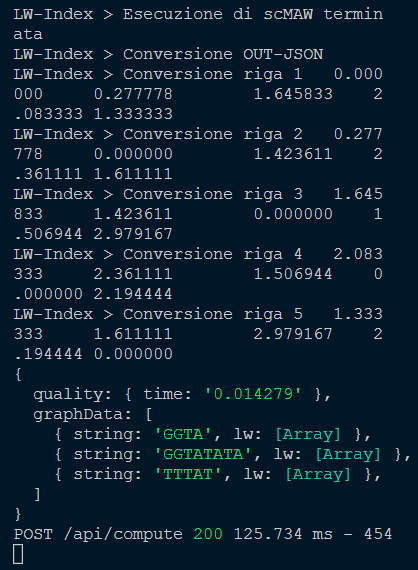
\includegraphics[width=4in]{Figure/console.png}}
    \caption{Anteprima di una porzione del processo di computazione svolto dal server.}
    \label{fig:esempio}
\end{figure}


L'istruzione conclusiva \verb|res.json(responseData)| rappresenta la chiusura della richiesta e l'invio della risposta al client. A questo punto, il webserver rimarrà attivo e in attesa di nuove richieste da parte del client. Non eseguirà, in ogni caso, altre azioni in autonomia.

\subsection{Frontend e Webclient}

L'implementazione del frontend di una piattaforma web in React è dissimile rispetto ai metodi tradizioni di costruzione di siti web interattivi con tecnologie primitive come JavaScript. React, per definizione, è un framework per JavaScript che adotta una filosofia a componenti. Ogni elemento sulla pagina viene interpretato logicamente come un componente funzionale della piattaforma, dipendente o meno rispetto ad un componente padre, e contenente o meno uno o più componenti figli. 

I componenti React sono estremamente versatili e poliedrici, in grado di assumere connotazioni particolarizzanti in funzione degli obiettivi dello sviluppatore. 

Oltre a React, la marcatura della piattaforma sarà costruita tramite HTML e CSS. 

Per quanto si vorrebbe dare una spiegazione ampia e dettagliata di ogni singolo aspetto dell'implementazione del frontned, non è possibile data l'enorme mole di codice, che si attesta sull'ordine delle migliaia di righe al netto dei file autogenerati dal processo di installazione. Per questo motivo, il codice sorgente è liberamente e gratuitamente consultabile su GitHub. \cite{lwIndexGithub}

\vspace{3mm}

Il sistema dovrà essere fornito di una dashboard interattiva e un menù laterale che permetta di effettuare operazioni. Le operazioni, essenzialmente, avranno il compito di alterare il contenuto della dashboard, e di conseguenza modificare lo stato dell'applicazione.

\newpage

\subsubsection{Trasmissione globale delle informazioni}

L'applicativo è strutturato a componenti funzionali, più o meno indipendenti l'uni dagli altri. 

Tuttavia, tutti fanno riferimento ad un singolo componente per la trasmissione globale di dati e informazioni; altresì, questo stesso componente è responsabile della generazione di nuovi componenti e, in generale, del corretto funzionamento dell'applicazione. 

L'intero applicativo è, ad un certo istante, un'istanza delle possibili configurazioni che il suddetto componente può assumere. Il componente in questione è chiamato \verb|App|. Fra le altre cose, il componente è responsabile della creazione dei grafici e della corretta renderizzazione del markup sulla pagina.

Se un qualsiasi componente ha necessità di spedire un dato, oppure propagare un'informazione, al resto dell'applicativo, si limiterà piuttosto a delegare al componente \verb|App| tale compito, specificando la natura della trasmissione e il contenuto del messaggio.

\vspace{3mm}

Di seguito viene riportata una porzione del componente \verb|App|. In generale, il componente è declinato da una moltitudine di funzioni, variabili e constanti in grado di alterare l'applicazione nel suo complessivo.

\begin{sexylisting}{App}
const [alertProps, setAlertProps] = ..
const [alertStatus, setAlertStatus] = ..
const [graphs, setGraphs] = ..
const [ability, setAbility] = ..
const [selectedAlgo, setSelectedAlgo] = ..

[..]
\end{sexylisting}

\subsubsection{Dashboard e gestione dello stato}

Il menù laterale prevede tre macrosezioni: \textbf{Operazioni}, \textbf{Algoritmo} e \textbf{Debug}.

\vspace{3mm}

\begin{itemize}
    \item La sezione \textbf{Operazioni} sarà l'area principale di interazione con l'utente. L'utente potrà creare nuove istanze di lavoro, analizzarle, eliminarle e svuota l'intera dashboard. Si osservi che 'tavolo di lavoro' e dashboard sono intercambiabili.
    \item La sezione \textbf{Algoritmo} fornisce informazioni critiche sull'algoritmo selezionato, permettendo inoltre di selezionarne di differenti. 
    \item La sezione \textbf{Debug} permette di generare una serie di grafici esemplificativi, riempiendo il tavolo di lavoro con quattro istanze popolate, e di accedere al codice sorgente dell'applicazione, che è open source.
\end{itemize}

Il componente \verb|Nav| governa il comportamento del menù laterale, distiguendo le operazioni esegubili in funzione dello \textbf{stato del sistema}. Il tool, infatti, ad un certo istante può avere solo uno dei due seguenti stati.
\begin{itemize}
    \item \textbf{SingleGraph}: stato di analisi. Per accedere a questo stato, è necessario che almeno un grafico (vuoto o meno) sia presente sul tavolo di lavoro, e che uno di questi grafici sia stato selezionato tramite "Analizza istanza" sul menù laterale, nella sezione Operazioni.
    \item \textbf{MultiGraph}: stato di \textit{default}. Ammette la creazione, rimozione e analisi dei grafici; la selezione di nuovi algoritmi; la generazione di esemplificazioni.
\end{itemize}

Le configurazioni dello stato dell'applicativo sono elaborate in un dato speciale definito \verb|AppStatusSet|. I componenti dell'applicativo possono richiedere cambiamenti di stato trasmettendo al componente \verb|App| un'opportuna richiesta. Inoltre, \verb|AppStatusSet| contiene informazioni sui grafici attivi: in questo modo, i cambiamenti di stato non produrranno modifiche accidentali (e potenzialmente distruttive) al tavolo di lavoro.

\begin{sexylisting}{AppStatusSet}
const [appStatusSet, setAppStatusSet] = 
  useState<AppStatusSet>({
    appStatus: AppStatus.__MultiGraph,
    graph: {
      ...BlankGraph,
	  algo: selectedAlgo,
    },
  });
\end{sexylisting}

\vspace{3mm}

L'operazione di creazione di nuove istanze di lavoro genererà dei quadranti svuoti, identificati da un indice incrementale. Le istanze sono analizzabili o eliminabili. Come accennato in precedenza, creare o distruggere grafici è direttamente legato allo stato dell'applicativo; motivo per cui, alla richiesta di creazione o eliminazione di grafici, il componente \verb|Nav| trasmetterà la richiesta al componente \verb|App|, che eventualmente procederà ad alterare lo stato dell'applicazione. 

\vspace{3mm}

In particolare, la richiesta di creazione ed eliminazione di grafici, assieme alla richiesta di analisi di grafici, sono fra le uniche che richiedono al componente \verb|App| di ridisegnare l'interfaccia utente, e cioè modificare direttamente l'aspetto esteriore dell'applicazione.

\vspace{3mm}

In alternativa, il tavolo di lavoro è svuotabile di tutte le sue istanze di lavoro. Questa operazione non riporta a zero l'indice identificativo dei grafici, al fine di tener traccia delle attività dell'utente.

\subsubsection{Fase di analisi delle istanze di lavoro}

E' possibile analizzare le istanze di lavoro a prescindere dal loro stato; di conseguenza, un'istanza è analisi anche se non ancora popolata da stringhe. Analizzare un'istanza trasformerà il tavolo di lavoro generale in un tavolo di lavoro specifico per l'istanza in analizi. Da questa schermata, è possibile effettuare la maggior parte delle operazioni previste dalle funzionalità ad alto livello indicate in precedenza.

\vspace{3mm}

Se l'istanza in analisi è neonata o non popolata, il semispazio superiore della schermata sarà occupato da due assi esenti da curve. In alternativa, se l'istanza è stata precedentemente popolata o si richiede una nuova computazione in essere, il semispazio sarà occupato da un grafico ricco di tante curve quante le stringhe immesse nella parte sinistra del semispazio inferiore della schermata di analisi.

\vspace{3mm}

D'altro canto, il semispazio inferiore consta - nel lato sinistro -  di una sezione di immissione, rimozione e modifica delle stringhe in input. E' possibile aggiungere o rimuovere form di input tramite il pulsante "Inserisci". Accanto ad ogni form di input, sarà presente - oltre ad un pulsante per verificare la validità, e dunque aggiungere, la stringa digitata - un tasto per rimuovere il form dalla schermata, e un quadrante che indicherà la validità della stringa immessa. 

\vspace{3mm}

Difatti, algoritmi diversi ammettono stringhe composte a partire da alfabeti distinti. Nel caso dell'algoritmo predefinito scMAW, l'unico alfabeto consentito è $DNA$. In caso di immissione di una stringa non consentita, il quadrante si popolerà con una $X$ rossa; in alternativa, in caso di validità, il quadrante si popolerà con un $OK$ verde. Fino alla pressione del pulsante "Aggiungi", il quadrante sarà occupato da un $?$.

\vspace{3mm}

Il lato destro del semispazio inferiore proporrà una serie di informazioni circa la natura e la composizione dell'insieme di stringhe $S$ da dare in pasto all'algoritmo. D'altro canto, un grafico relativo alla qualità (in termini di secondi) della computazione

\subsubsection{Selezione e integrazione degli algoritmi}

La sezione Algoritmi prevede, fra le altre cose, una voce per selezionare l'algoritmo da usare. Alla pressione, un alert personalizzato si presenterà all'utente, oscurando il restante contenuto della pagina e portando l'attenzione dell'utilizzare al selezione. L'alert conterrà una lista di algoritmi, ognuno presentato come bottone interattivo. L'interazione con uno qualsiasi dei bottoni presenti condurrà ad un cambio di stato dell'applicazione, per il quale il sistema sarà notificato di impiegare l'algoritmo selezionato.

\vspace{3mm}

Una volta selezionato l'algoritmo, la piattaforma sarà in grado di riformulare le modalità di computazione alla prossima richiesta. E' dunque possibile tornare (o avviare) una fase di analisi e procedere ad una nuova computazione. Quest'ultima verrà eseguita impiegando l'ultimo algoritmo selezionato.

\vspace{3mm}

La selezione di algoritmi è governata dal componente \verb|AlgoSelector| il quale predispone un array di elementi (quali i pulsanti di selezione degli algoritmi), ognuno dei quali interagibili al \textit{click}. Ogni click produce un cambiato di stato: in particolare, viene lanciata la funzione \verb|setSelectedAlgo()| per comandare all'hub \verb|App| di trasmettere all'intero sistema le proprietà del nuovo algoritmo.

E' interessante osservare come l'array di algoritmi viene generato. 

\begin{sexylisting}{AlgoSelector}
ALGOS.forEach((algo) => {
  temp.push(
    <div
      onClick={() => {
		[..] props.setSelectedAlgo(algo);
	  }}
	  className='selector'
	>
	  {algo.name}
    </div>
  );
});
\end{sexylisting}

Nel componente in esame, così come nel resto del sistema, \verb|ALGOS| rappresenta logicamente gli algoritmi disponibili. Se uno svluppatore volesse integrare il proprio algoritmo nel tool, sarebbe sufficiente aggiungere una nuova entry nel seguente array, indicando le proprietà \verb|name| (nome dell'algoritmo), \verb|info| (informazioni riguardanti il funzionamento dell'algoritmo -- ad esempio, le strutture dati utilizzate) e \verb|abbr| (un nome alternativo sufficientemente corto).

\begin{sexylisting}{ALGOS: Algo[ ]}
const ALGOS: Algo[] = [
  {
    name: 'Sequence Comparison by Absent Words',
	info: "[..]",
	abbr: 'scMAW',
  },
  {
    name: 'Test Algo',
	info: 'Informazioni Test Algo',
	abbr: 'test',
  },
];
\end{sexylisting}

Posto che il server sia popolato dai file necessari (rif. Capitolo 5.1) per eseguire l'algoritmo, il sistema sarà in grado di riconoscere immediatamente la presenza di un nuovo algoritmo fra le sue file, e permettere dunque nuovi confronti fra stringhe impiegandolo.

\newpage

\subsection{Interfaccia utente}

L'interfaccia di LW Index è spartana e alterna colorazioni scure a tonalità più chiare, al fine di mettere in risalto gli elementi interagibili della UI.

\subsubsection{Generazione automatica di grafici esemplificativi}

La voce \textit{Genera esemplificazioni} del menù laterale è particolarmente utile per avere un'anteprima del funzionamento dell'applicativo. Alla pressione, infatti, il tool autogenererà quattro grafici con dati casuali, simulando il processo di elaborazione di cui si occupa il server. Proprio perché i dati sono casuali, il riavvio dell'applicazione resetterà i parametri che generano i grafici, creandone di nuovi ogni volta.

\begin{figure}[ht!]
    \centering
    \tmpframe{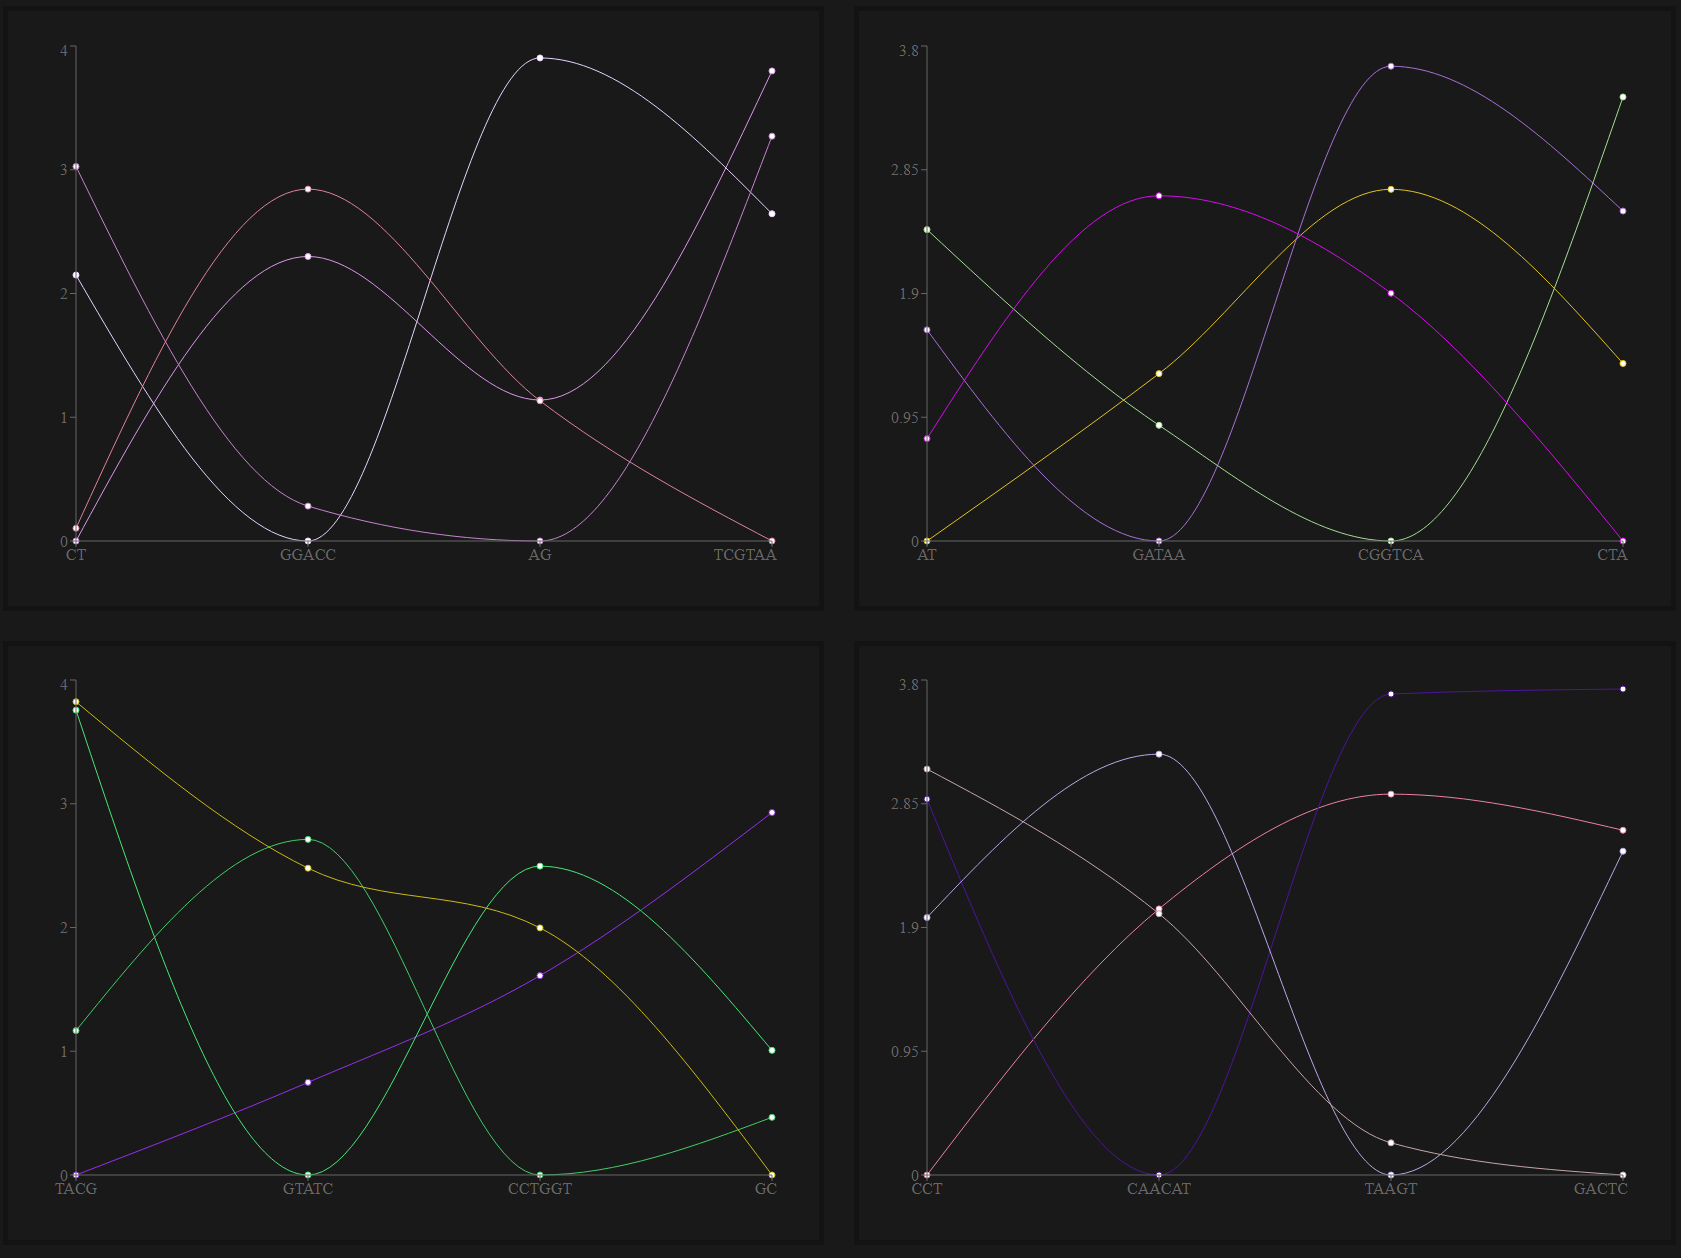
\includegraphics[width=6in]{Figure/esempi.png}}
    \caption{L'operazione di debug "Genera esemplificazioni" riempie il tavolo di lavoro con grafici casuali come in figura.}
    \label{fig:esempio}
\end{figure}

\begin{figure}[ht!]
    \centering
    \tmpframe{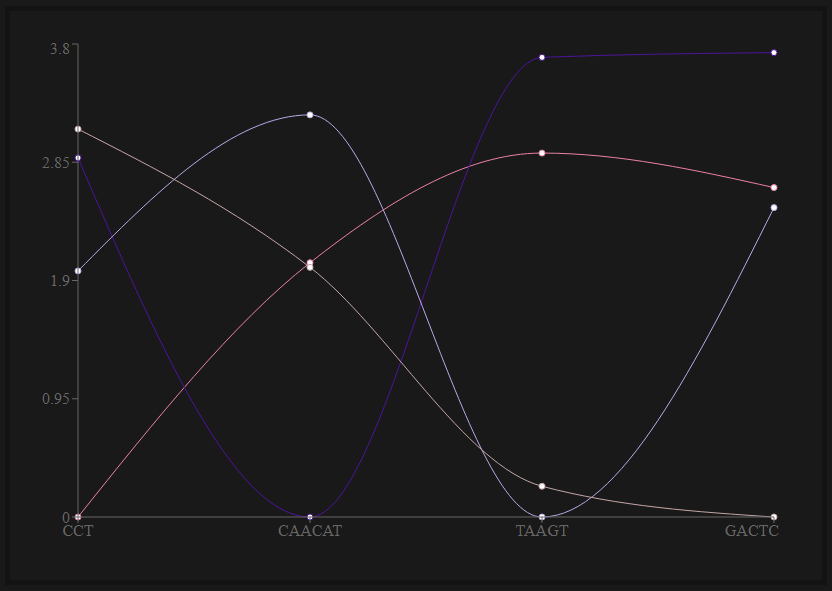
\includegraphics[width=6in]{Figure/singoloEsempio.png}}
    \caption{Dettaglio di un singolo grafico esemplificativo autogenerato tramite operazioni di debug.}
    \label{fig:esempio}
\end{figure}

\subsubsection{Selezione degli algoritmi}

L'interfaccia di selezione di algoritmi è costituita da un semplice alert composto da bottoni interattivi. Ogni bottone rappresenta uno degli algoritmi selezionabili, ordinati lessicograficamente. La pressione di un bottone produrrà un significativo cambio di stato nell'applicativo.

\begin{figure}[ht!]
    \centering
    \tmpframe{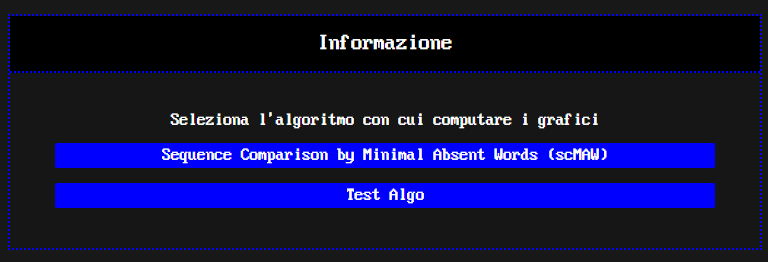
\includegraphics[width=5.5in]{Figure/selectAlgo.png}}
    \caption{Gli algoritmi sono elencati per nome. Nell'esempio in figura, sono disponibili solo due algoritmi.}
    \label{fig:esempio}
\end{figure}

\clearpage

\subsubsection{Schermata di analisi}

La schermata di analisi è del tutto bianca, per indicare all'utente che si è in una fase dell'utilizzo dell'applicazione genuinamente interattiva. La maggior parte delle componenti sulla schermata sono interagibili e produrranno significativi cambi di stato o l'invocazione del webserver per l'esecuzione di operazioni nel backend.

\begin{figure}[ht!]
    \centering
    \tmpframe{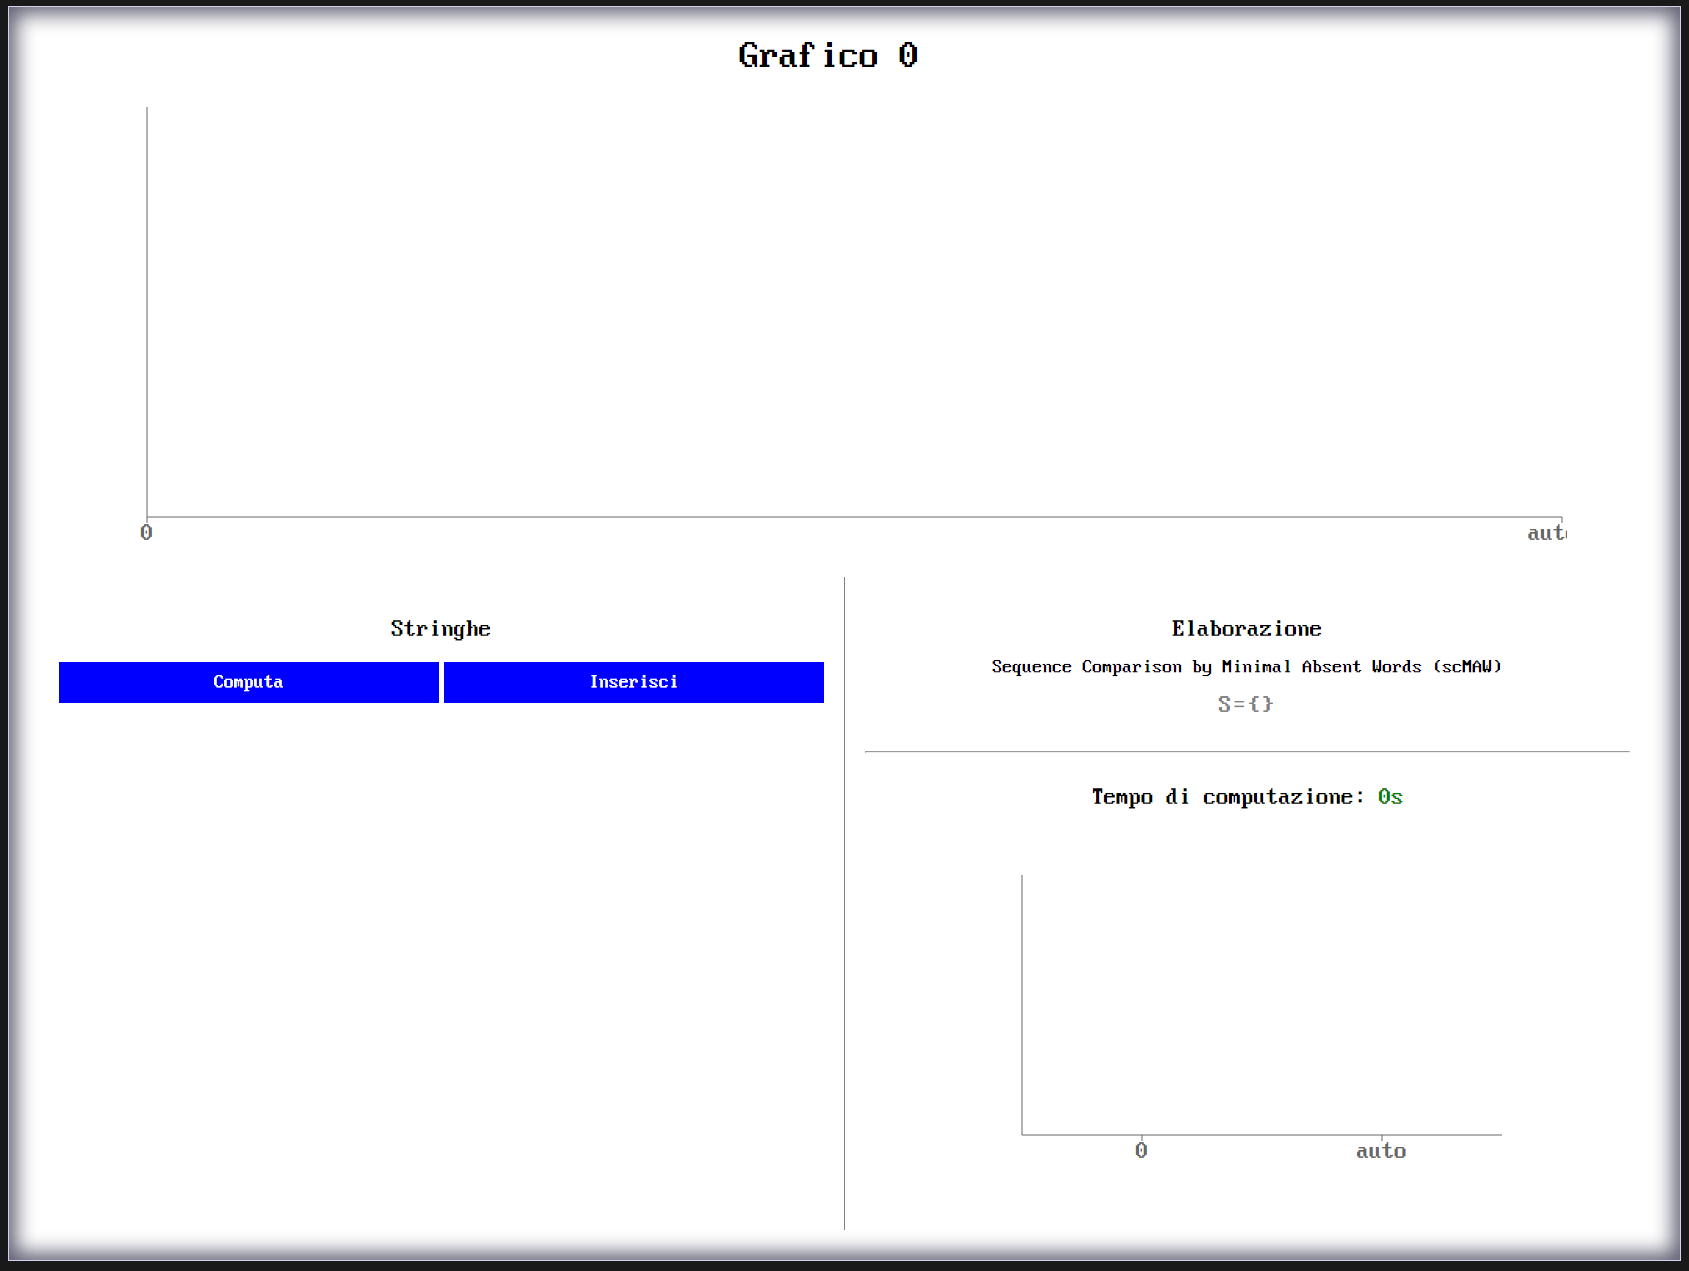
\includegraphics[width=6in]{Figure/analisi.png}}
    \caption{La fase di analisi prevede una schermata bianca divisa in due semispazi, come in figura.}
    \label{fig:esempio}
\end{figure}

\clearpage

\subsubsection{Stringhe in input}

Due schermate in particolare permettono di tener traccia e di manipolare le stringhe in input. E' fondamentale che l'utente sia in grado di discernere con rapidità le stringhe ammesse, non ammesse o non ancora verificate; d'altro canto, è importante che salti all'occhio la possibilità di modificare, aggiungere o alterare l'insieme di stringhe in input, motivo per cui sono state utilizzate tonalità uniche, disponibile ersclusivamente nella schermata di analisi.

\begin{figure}[ht!]
    \centering
    \tmpframe{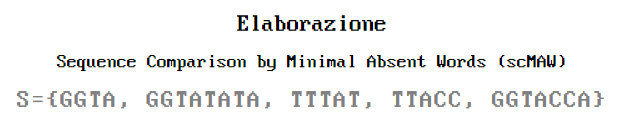
\includegraphics[width=6in]{Figure/stringheInsieme.png}}
    \caption{La successiva computazione che l'utente avvierà avrà come input l'insieme $S={GGTA, GGTATATA, TTTAT, TTACC, GGTACCA}$ delle stringhe. L'algoritmo selezionato è indicato col suo nome completo e un suo eventuale acronimo.}
    \label{fig:esempio}
\end{figure}

\begin{figure}[ht!]
    \centering
    \tmpframe{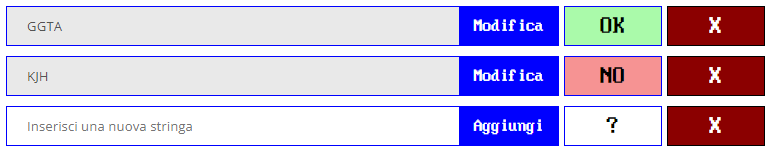
\includegraphics[width=6in]{Figure/stringhe.png}}
    \caption{Nell'esempio in figura, l'utente ha generato tre form di input, digitando $GGTA$ nel primo, $KJH$ nel secondo e lasciando vuoto il terzo. Ha, inoltre, premuto "Aggiungi" (sostituito adesso da "Modifica") nei primi due form. Il primo risulta valido, e cioè composto da lettere amesse dall'alfabeto; il secondo, invece, no. Poiché solo una stringa valida è stata immessa, l'utente non potrà computare alcun confronto da stringhe.}
    \label{fig:esempio}
\end{figure}

\newpage

\subsubsection{Grafici illustrativi}

I grafici offerti sono fondamentalmente due: il \textit{grafico di validità} degli indici LW, che permette di assicurare la robustezza dell'algoritmo selezionato; e il \textit{grafo di qualità} dell'algoritmo, che permette di confrontare, sfruttando il tempo di computazione come parametro, gli algoritmi impiegati.

\begin{figure}[ht!]
    \centering
    \tmpframe{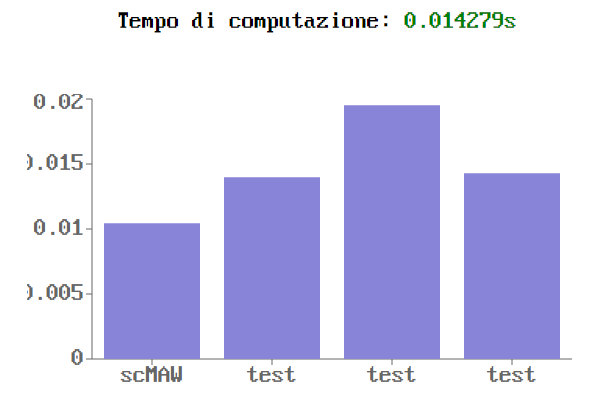
\includegraphics[width=5in]{Figure/computo.png}}
    \caption{L'utente ha effettuato 4 computazioni. L'ultima computazione ha impiegato $0.014279$ secondi. Le prime tre computazioni sono state effettuate con l'algoritmo $scMAW$, mentre le restanti tre con l'algoritmo $test$. E' possibile determinare la qualità degli algoritmi proposti in maniera visiva; d'altro canto, insiemi di stringhe in input più vasti sarebbero in grado di produrre dati più significativi.}
    \label{fig:esempio}
\end{figure}

\begin{figure}[ht!]
    \centering
    \tmpframe{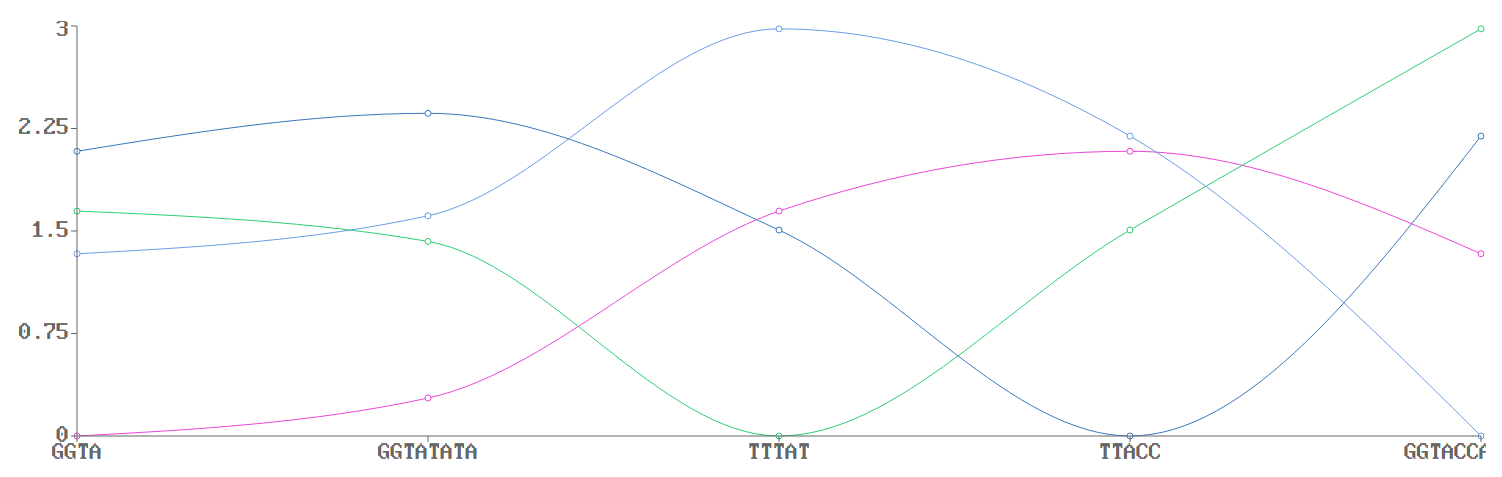
\includegraphics[width=6in]{Figure/grafico.png}}
    \caption{Esempio di grafico di validità generato dal tool.}
    \label{fig:esempio}
\end{figure}

\newpage

\subsubsection{Menù laterale}

Il menù laterale della piattaforma è stato progettato per essere quanto più usabile e funzionale possibile. La pressione diretta di una voce del menù coincide con la pressione del testo presente sulla voce stessa; in generale, il menù laterale può essere visto come una tabella, composta da tante voci quante le operazioni possibili, più gli header (come ad esempio "Operazioni", o "Algoritmo") che non risultano interagibili. L'hover del mouse su una qualsiasi voce interagibile causerà un cambio di colore del testo di quest'ultima, passando da bianco ad azzurro.

\begin{figure}[ht!]
    \centering
    \tmpframe{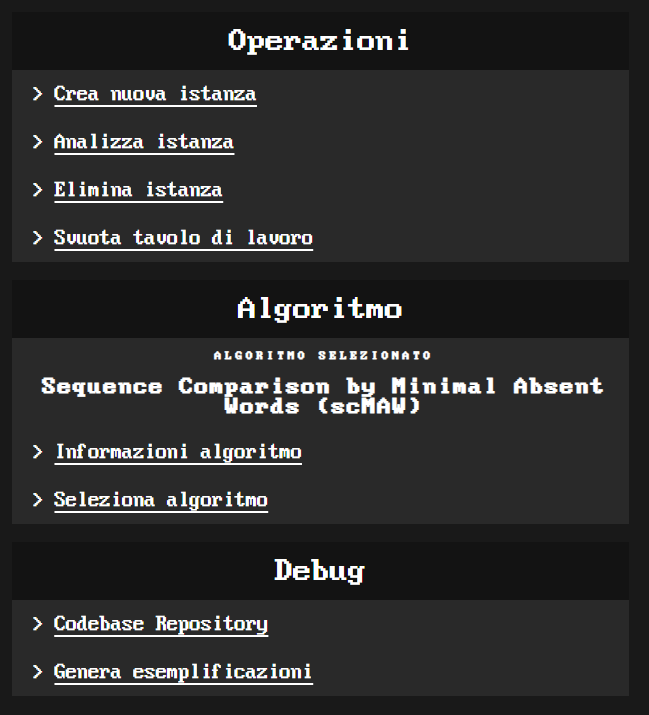
\includegraphics[width=5in]{Figure/menu.png}}
    \caption{Menù laterale della piattaforma.}
    \label{fig:esempio}
\end{figure}

\newpage

\subsubsection{Generazione di nuove istanze}

La creazione di nuove istanze di lavoro produrrà quadranti vuoti. Ogni quadrante sarà contrassegnato da un ID (detto \textit{GID}, ossia \textit{Graph ID}), il quale sarà stampato al centro del quadrante. Questi quadranti sono abilitati ad entrare in fase di analisi ed eliminazione.

\begin{figure}[ht!]
    \centering
    \tmpframe{
\includegraphics[width=6in]{Figure/graficiVuoti.png}}
    \caption{L'utente ha generato due grafici vuoti, che adesso popolano il tavolo di lavoro.}
    \label{fig:esempio}
\end{figure}